% Ejemplo del uso de la template para escribir tesis/memorias de la Universidad Diego Portales.
%
% Eviar bugs a: Adín Ramírez, adin.ramirez (at) mail.udp.cl

% Puede generar borradores si omite la opción "final" de la clase.
% \documentclass{udpthesis}
\documentclass[final]{udpthesis}

% Establecemos el sistema para uso del español
% Babel ya esta cargado dentro de updthesis
\usepackage[T1]{fontenc}%    output
\usepackage[utf8]{inputenc}% input
\usepackage{lmodern}

% Leyendas
\usepackage[font=footnotesize,labelfont=bf,labelsep=period]{caption}

% Agregue acá otros paquetes que le sean de utilidad
% Matemáticas
\usepackage{amsmath}

% Gráficos
\usepackage{graphicx}
\usepackage[font=footnotesize,labelformat=simple]{subfig}
% Cambiamos el formato de las leyendas: finalizan en punto, y en negrita.
\captionsetup{labelsep=period,labelfont=bf}
% Habilitamos el uso de paréntesis al citar las figuras con subfiguras dentro, e.g., Fig. 1(a)
\renewcommand\thesubfigure{(\alph{subfigure})}
\renewcommand\thesubtable{(\alph{subtable})}
\newcommand{\subfigureautorefname}{\figureautorefname}

% Código
% Para generar código fuente usar listings.sty
%\usepackage{listings}
%\usepackage{tikz}
%\lstset{
%  language=[LaTeX]TeX,
%  breaklines=true,
%  basicstyle=\tt\scriptsize,
%  keywordstyle=\color{blue},
%  identifierstyle=\color{magenta},
%  commentstyle=\color{green!40!black},
%  % frame 
%  frame=tb,
%  captionpos=t,
%  xleftmargin=1em,
%  numbersep=0.3em,
%  numbers=left,
%  framexleftmargin=1.1em,
%  framexrightmargin=0pt,
%  % additional letters for accents in spanish
%  literate=%
%    {á}{{\'{a}}}1
%    {é}{{\'{e}}}1
%    {í}{{\'{i}}}1
%    {ó}{{\'{o}}}1
%    {ú}{{\'{u}}}1
%    {ñ}{{\~{n}}}1
%    {Ñ}{{\~{N}}}1
%}
%
%\renewcommand{\lstlistingname}{Código}% Listing -> Código
%\DeclareCaptionFormat{listing}{\rule{\dimexpr\linewidth\relax}{0.4pt}\par\vskip1pt#1#2#3}
%\captionsetup[lstlisting]{format=listing,singlelinecheck=false, margin=0pt,position=bottom}

% O para generar algoritmos en pseudocódigo usar algpseudocode.sty
%\usepackage{algorithm}
%\usepackage{algpseudocode}
%\makeatletter
%\renewcommand{\ALG@name}{Algoritmo}% Algorithm -> Algoritmo
%\makeatother
%\captionsetup[algorithm]{font=footnotesize,labelsep=period}

% Referencias (este paquete ordena y comprime las referencias)
\usepackage{cite}

% Un paquete para generar texto. REMUEVA ESTE PAQUETE AL UTILIZAR ESTA PLANTILLA.
\usepackage{blindtext}


% Establecemos el tema a utilizar. 
% Debe existir el archivo udpthesisEIT.sty en su sistema TeX para poder utilizarlo.
% Por ejemplo, para utilizar el tema de magíster de la EIT deben de utilizar
% \udptheme{EIT-MS}
\udptheme{EIT}

\newcommand{\dd}[1] {\textbf{\textcolor{blue}{[dd:] #1}}}
\newcommand{\os}[1] {\textbf{\textcolor{red}{[os:] #1}}}

\begin{document}
%% Inicio de la portada
\frontmatter

% Título del tema (no más de 12 palabras)
\title{Diseño e implementación de algoritmo de asignación dinámica de celdas para la Internet Industrial de las Cosas}
% para precisar aún más su tema, use un subtítulo
%\subtitle{Subtítulo explicativo del tema}

% El autor(es) de la tesis
\author{Oscar Leonardo Solis}
\email{oscar.solis@mail.udp.cl}% utilice un correo que revise después de graduado

% o una lista de autores separados con comas
%\author{Juan Bar, José Foo}
%\email{juan.bar@mail.udp.cl, jose.foo@mail.udp.cl}

% Fecha a aparecer en la tesis
\date{2016}

% Profesor guía
\professor{Diego Dujovne}
% Comité
\committee{Luis Loyola}{Luciano Ahumada}

% Dedicatoria
\dedicatory{Dedicado a todas las personas que se han cruzado en mi camino, a pesar de que algunas ya no estén, y que directa o indirectamente han participado en mi proceso de formación.}

% Agradecimientos
\acknowledgment{Quiero agradecer a mi familia, amigos, y profesores.}

% Abstract en inglés
\abstract{%<- evita nueva linea en el abstract
This first stage presents a study of the state of the art in wireless sensors area, which are being increasingly used in industries and factories, in a lot of different applications. The use of this kind of sensors has been exponentially growing according to the complexity of industrial processes.

Wireless networks are an emerging field that encompasses the development of different areas of information technologies, telecommunications, and inclusion of different disciplines such as agriculture, medicine, biology, mechanics, etc. Components, topologies, standards, applications, difficulties and possible solutions: key concepts are addressed.

When someone decides to use a wireless network, the decision is taken hoping its features must be equal or greater than a wired network, so this is the basis for deciding to use a wireless network. This implies that one must have wired network standards such robustness, latencies within acceptable parameters, and also the benefits of a wireless network, such as the need for flexibility and minimal maintenance.

In this chapter we will work with those based on TSCH wireless networks. Industrial application networks whose architecture allows adjusting the distribution of resources as frequency and time. Because the operating environment of these networks is hostile, and constantly changing, these resources must be constantly adjusted to new conditions.

The scope of this present work is to propose an improvement to the scheduling function zero (SF0) which is based on neighbor to neighbor scheduling method.



}
% Resumen
\resumen{%<- evita nueva linea en el resumen 
Esta primera etapa presenta un estudio sobre el estado del arte en el área de sensores inalámbricos, cuya utilización ha ido creciendo exponencialmente a medida que se han vuelto mas complejos los procesos industriales.

Las redes inalámbricas conforman un campo emergente que engloba el desarrollo de distintas áreas de las tecnologías de la información, telecomunicaciones, e inclusión de distintas disciplinas como la agricultura, medicina, biología, mecánica, etc. Se abordarán los siguientes conceptos principales: componentes, topologías, estándares, aplicaciones, dificultades y posible soluciones.

A la hora de decidir si utilizar una red inalámbrica, se debe tener presente que sus características deben ser iguales, o superiores a las de una red cableada, por lo tanto esta es la base para decidir utilizar una red inalámbrica. Esto implica que se debe cumplir con los estándares de una red cableada como la robustez, latencias dentro de parámetros aceptables, y además de los beneficios de una red sin cables, como son la flexibilidad y la necesidad de mantenimiento mínimo.

En este capítulo se trabajará con las redes inalámbricas basadas en la tecnología "Time Slotted Channel Hopping" (TSCH por sus siglas en inglés), de aplicación industrial y cuya arquitectura permite ajustar la distribución de los recursos como frecuencia y tiempo. Dado que el entorno de funcionamiento de estas es cambiante y hostil, estos recursos deben estar constantemente ajustándose a las nuevas condiciones. Este trabajo tiene como objetivo proponer una solución a esta asignación dinámica de recursos.

Este trabajo de investigación tiene como objetivo proponer una mejora a la función de calendarización cero (SF0) la cual se basa en el método de calendarización ``vecino a vecino''.


}

% Generamos la portada
\makecover

% Indices y listas
\tableofcontents% tabla de contenido
\listoftables%    índice de tablas
\listoffigures%   índice de figuras
% puede agregar otras listas o índices acá de ser necesario



% Inicio del contenido
\mainmatter

% Capítulos y secciones del documento
% Aca se incluyen los archivos con el texto de los capitulos
% Incluyo el archivo cap-intro.tex
\chapter[Introducción]{Introducción}
\label{ch:intro}

\section{Motivación}
Los sensores durante muchos años han sido herramientas muy útiles en el control de procesos, ya que permiten sensar magnitudes físicas involucradas en los procesos en tiempo real, y tener una referencia de lo que está ocurriendo, sin tener que esperar a que finalice un proceso para evaluar el resultado.
A medida que los procesos se tornan más complejos, se ha llegado a requerir mayor cantidad de medios para extraer información, lo cual entorpece el desarrollo, debido a las grandes cantidades de cables necesarios para alimentar, y extraer información de sensores. Es por esto que se han enfocado los esfuerzos en eliminar estos cableados, lo cual trae un problema: encontrar el equilibrio entre duración de fuente de energía, versus la cantidad de información capaz de manejar, además de la confiabilidad requerida en este tipo de aplicaciones. Esto ha dado pie al surgimiento de sistemas de redes de sensores inalámbricos ó WSN (Wireless Sensor Network), que se compone por miles, e incluso millones de sensores, que llamaremos nodos, y que son capaces de generar información, procesarla y transmitirla con recursos energéticos limitados.
La constante evolución de esta rama de sensores ha abierto un abanico de posibilidades de aplicación, por ejemplo la fabricación de vehículos, domótica, monitorización ambiental, salud, áreas comerciales y militares. \cite{dujovne20146tisch}
En este documento se expone un estudio acerca de las redes TSCH, principales términos de las redes de sensores, aplicaciones, y los principales estándares presentes, para luego abordar las redes inalámbricas usando IPv6 bajo el estándar IEEE802.15.4e, y herramientas de simulación.

\section{Fundamentos de redes de sensores}

\subsection{Definición}
Una red de sensores inalámbricos es una red de pequeños dispositivos situados en una determinada localización física, capaces de interactuar con esta red.
Las redes de sensores se diseñan específica, y deben distribuirse en un área determinada. Estos pueden ser estacionarios o móviles.
Los nodos contruyen una red Ad-Hoc, donde los dispositivos que la componen son capaces de realizar enrutamiento entre ellos. Para conseguir esto, estos dispositivos se autoconfiguran sobre una topología determinada, y según se vaya modificando la cantidad y localización de los dispositivos, se va actualizando, y re enrutando dinámicamente según lleguen nuevos dispositivos, o se retiren.
Existe una variedad de aplicaciones en las que se puede utilizar redes de sensores inalámbricos, entre las que se pueden destacar son las siguientes:

\begin{itemize}
    \item Aplicaciónes médicas:
    \begin{itemize}
        \item Monitorear signos vitales.
        \item Diagnosticar.
        \item Suministrar medicamentos.
        \item Control ambiental.
        \end{itemize}
    \item Aplicaciones medioambientales:
    \begin{itemize}
        \item Determinar parámetros como luz, temperatura, radiaciones.
        \item Detectar incendios forestales
        \item Monitorear contaminación
        \item Censar velocidad y temperatura de vientos.
        \end{itemize}
        
        \newpage
    \item Aplicaciónes en maquinaria:
    \begin{itemize}
        \item Medir movimientos y vibraciones.
        \item Censar temperatura, ruidos.
        \item Estimar magnitudes como velocidad, aceleración, dirección, etc.
        \end{itemize}
    \end{itemize}


Para cada aplicación es necesario que los sensores sean capaces de entregar un desempeño confiable, por ejemplo en aplicaciones médicas, es necesario que sea fiable la transmisión de datos, debemos tener presente que el monitoreo de signos vitales es crítico en una persona, y no se debe dar espacio a incertidumbres. Caso similar para la aplicación en monitoreo medioambiental, donde se necesita que los sistemas sean capaces de alertar de un posible incendio lo mas pronto posible. Para el caso de aplicaciones en maquinaria, tambien es necesario tener la información lo antes posible para prevenir posibles daños frente a situaciones de sobreexigencia, temperatura o fatiga de materiales.

Cuando se trabaja con estas redes, es necesario que identificar que componentes se necesita utilizar, para tener datos precisos y correctos. A continuación se muestran los componentes disponibles para utilizar en una implementación de redes de sensores.




\subsection{Elementos}

\begin{itemize}
    \item Sensores: Existen de diferente naturaleza, su función es capturar información del entorno, y codificarla en información digital.
    \item Nodo sensor: O también llamados “Motes” en algunos países, o procesadores de radio, su función es tomar los datos del sensor a través de sus entradas de datos, y enviarla o propagarla. Este es el conjunto de nodo transmisor y sensor o sensores.
    \item Nodo: Es un sensor, puede o no contener procesador de radio, cuando este es el caso, pasa a ser un nodo sensor.
    \item Puerta de enlace:Punto de conexión entre los nodos, y una red TCP/IP.
    \item Estación base: Etapa, o sistema el cual recibe o recopila los datos, puede ser un computador, u otro nodo de la red.
\end{itemize}

 Los elementos descritos deben ser capaces de interactuar entre sí para intercambiar información. Para esto, es necesario que cada componente utilice un lenguaje estándar para comunicarse entre si, esto permite plantear el concepto de estándares de comunicación, el cual se explicará a continuación.



\subsection{Estándares}

Al iniciarse el desarrollo de las redes inalámbricas, cada fabricante tenia sus propios métodos y lenguajes para interconectarse con otros dispositivos fabricados por el mismo, esto funcionaba muy bien para sus propios dispositivos, pero no así para los dispositivos distribuidos por otro fabricante. Por otro lado, los clientes de estos fabricantes debían estar dispuestos a adquirir solamente equipos de un solo fabricante. Esto traía malas prácticas en cierto modo monopólicas.

Entrando en el año mil novecientos noventa y siete, el Instituto de Ingenieros Eléctricos y Electrónicos IEEE, tomando características de sistemas de comunicación junto a un grupo de distintos fabricantes de sistemas de telecomunicaciónes, generó y estableció un protocolo universal, el cual los fabricante podían utilizar para manufacturar tanto dispositivos de emisión, como de recepción. Estos dispositivos debían poder interactuar con dispositivos de otros fabricante que cumplieran el mismo estándar. Esto dió origen al estándar 802.11. \cite{crow1997ieee}

Conforme pasan los años, los sistemas de telecomunicaciones se hacen mas capaces, y las exigencias se incrementan, por lo tanto, los protocolos quedan obsoletos, es por esto que se hace necesario que se actualicen los estándares, agregándoles características, y reemplazando otras. Esto da origen a las revisiones, las cuales incluyen mejoras junto al estándar base, y se denominan añadiendole una identificación al protocolo como fue el caso de 802.11a, cuya mejora posteriormente fue añadida por completo al protocolo 802.11, manteniendo este mismo nombre final.

Dicho esto, se asume que las redes inalámbricas deben basarse en estándares, el cual debe alcanzar un equilibrio entre velocidad de transmisión, cobertura y coste energético por paquete enviado, para conseguir esto, se elaboró una pila de protocolos, concepto que materializa lo que abarca la idea de una conexión entre distintos dispositivos. Esta pila define los distintos roles al momento de establecer una comunicación de cualquier tipo, roles que deben desempeñarse correctamente, de lo contrario no sería posible entablar una comunicación.

Este documento se basa en la implementación por parte de la IETF del protocolo IP versión 6 sobre una red ``Time slotted channel hopping'', TSCH por sus siglas en ingles, nombrado también bajo estándar IEEE802.15.4e. Una red TSCH es una red capaz de ajustar su canal de comunicación a un espacio de tiempo asignado por un calendarizador, el que puede ser implementado utilizando diferentes algoritmos, los cuales serán abordados en este documento.

\subsubsection{Estándares relacionados}

Es necesario destacar que las redes TSCH han sido desarrolladas por distintos organismos, los cuales han dado una aplicación diferente según el área de la industria. Por un lado tenemos las redes industriales TSCH WirelessHART, y por otro lado tenemos las redes ISA100.11a. Ambas redes se basan en el estándar IEEE802.15.4, el cual opera en una frecuencia de 2.4 Gigahertz. Ambos son utilizados en una amplia gama de aplicaciónes industriales, sobre todo en procesos de automatización de procesos, y de plantas de producción.
Ambos estándares son usados como LoWPAN (redes inalámbricas de área personal de baja tasa de transferencia, por sus siglas en inglés). ISA100.11a usa una capa MAC la que es una versión modificada de la capa MAC utilizada por WirelessHART. Ambas utilizan el mismo mecanismo para el transporte de datos desde, y hasta la puerta de enlace. Como ambas tecnologías operan en muy baja potencia, la vida de sus baterías es extensa.
Sus radios utilizan DSSS(ampliación de espectro por secuencia directa por sus siglas en inglés) para permitir la coexistencia del mismo espectro de frecuencia sin interferirse de ninguna manera entre ellas

\begin{figure}
\centering
\graphicspath{ {imagenes/} }
\begin{minipage}{.5\textwidth}
  \centering
  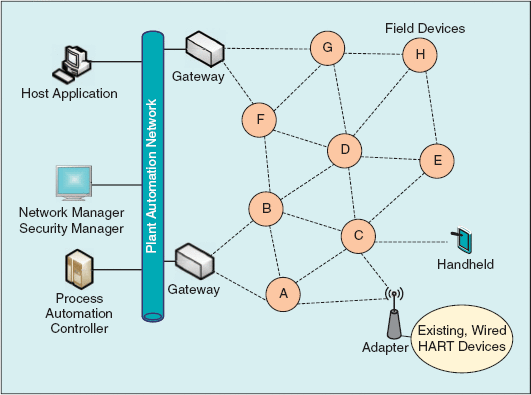
\includegraphics[width=.9\linewidth]{HART.png}
  \captionof{figure}{Imagen de una red WirelessHART}
  \label{HART}
\end{minipage}%
\begin{minipage}{.5\textwidth}
  \centering
  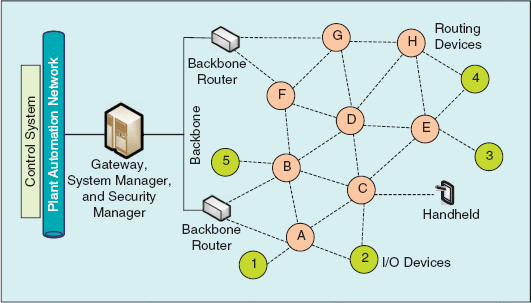
\includegraphics[width=.9\linewidth]{ISA100.png}
  \captionof{figure}{Imagen de una red ISA100.11a}
  \label{ISA100}
\end{minipage}
\end{figure}

Las imágenes \ref{HART}, y \ref{ISA100} muestran las similitudes y diferencias entre estos dos tipos de estándares.\cite{petersen2011wirelesshart}




A pesar que el estándar ha tenido dos revisiones, el estándar de la capa física no ha cambiado, sino que se ha incorporado una nueva capa MAC como complemento al modelo IEEE802.15.4 \cite{RFC7554}, siendo esta capa MAC ahora sincrónica y que asigna recursos por frecuencia y tiempo de manera simultánea. \cite{watteyne2015using}

La pila de protocolos propuesta por el grupo de trabajo 6TiSCH de la IETF, IPv6 sobre IEEE802.15.4e. protocolo que permite transmitir a una tasa de 250 kb/s en la banda de 2.4GHz, con un tamaño máximo de paquetes de 127 bytes. 

Cabe mencionar que este stack es utilizado en redes 6LoWPAN, equivalente al stack TCP/IP, pero adaptado a las redes (low powered and lossy networks) LLN por sus siglas en ingles. La imagen a continuación muestra las diferencias entre estos protocolos.

\begin{figure}[h]
\centering
\graphicspath{ {imagenes/} }
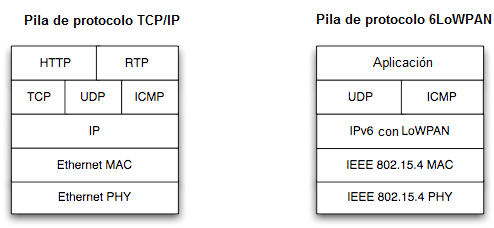
\includegraphics[width=0.9\textwidth]{stack.png}
\caption{Comparación entre stack 6LoWPAN y TCP/IP}
\label{stack}
\end{figure}

Los estándares mencionados son los que se usarán en este estudio, los que están contenidos en el protocolo 6TiSCH, el que se abordará a continuación.




\subsection{6TiSCH: IPv6 sobre redes IEEE802.15.4e TSCH}


Una red TSCH, es una red cuyo calendarizador es quien controla la comunicación, esto implica que el controlador asigna celdas de tiempo/frecuencia entre los nodos vecinos. Asignar múltiples espacios de tiempo a los mismos vecinos aumenta la cantidad de datos que estos nodos pueden intercambiar por segundo y reduce la latencia en la comunicación, pero por otro lado, esto implica que la radio de los nodos deberá estar encendida mas tiempo, aumentando el consumo energético promedio, y reduciendo la vida de su batería. Este documento aborda una perspectiva de la implementación del protocolo IP versión 6 sobre una red TSCH en la que se busca mejorar el desempeño de asignación de celdas de comunicación.


6TiSCH define un nuevo concepto global, el cual se llama “Matriz de distribución de canal/uso” (CDU) por sus siglas en inglés con una altura igual a la cantidad de frecuencias disponibles (indexados por una lista de distribución de canales) y un ancho en espacios de tiempo, que corresponde al “período” de la operación de calendarización de la red (indexados por una lista de acomodación de espacios, o ``slots'').

La matriz CDU puede ser particionada en trozos, los que llamaremos ``chunk'' por su nombre en inglés, un chunk es conocido globalmente por todos los nodos en la red para dar apoyo en el proceso de apropiación, el cual es una negociación entre nodos dentro de un dominio de interferencias.

Un nodo que se apropia de un chunk decide qué transmisiones van a ocurrir sobre las celdas en el chunk, dentro de su dominio de interferencia. Por último, un chunk representa una asignación de ancho de banda y puede ser visto como la generalización de un canal de transmisión en el dominio de tiempo/frecuencia.

\newpage
\subsubsection{Arquitectura}

6TiSCH está encausado en lograr el poco común hito de entregar una arquitectura que abarca múltiples estándares de diversas áreas dentro de de la IETF. La arquitectura 6TiSCH actualmente siendo diseñada con el objetivo de proveer altos PDR (Packet Delivery Rate por sus siglas en inglés) y latencia determinística de acuerdo a los protocolos de las redes de sensores inalámbricas industriales, como son ``WirelessHART'', y ``ISA100.11a''. Además, permite implementaciones de monitoreos de gran escala con el fin de cubrir el paradigma de internet industrial.

Con el fin de hacerlo escalable, y manteniendo el ancho de banda, la operación de ``6LoWPAN Neighbor Discovery (ND)'' se realiza dentro de la red, para eliminar la necesidad de realizar ``multicast'' e inundaciones, inherentes a la operación de la búsqueda de vecinos (ND) clásica de IPv6.

La experiencia de una WSN industrial da soporte a una aproximación centralizada, permitiendo un control total, y una optimización de la operación de la red desde un motor central de cómputo, con una “vista de dios”, la cual es llamada Administrador de red (Network manager en inglés), o Administrador de sistema, y que corresponde al Elemento de Cálculo del camino(PCE) en inglés, de la IETF. PCE considera todos los flujos y toda la capacidad de la red, calculando el grupo de pistas ``punto a punto'' (end-to-end) óptimo.

La arquitectura 6TiSCH debe cubrir todos los componentes tales como como seguridad y administración. Estos componentes afectan a todos los aspectos de las operaciones de la unidad, y cada una de las variadas técnicas que existen pueden ser relevantes para 6TiSCH. Sin embargo las limitaciones en memoria, CPU, ancho de banda, y latencia permiten implementar soluciones, pero son poco prácticas, y la necesidad de una red de alta escalabilidad y bajo mantenimiento motiva la implementación de sistemas autónomos.

6TiSCH apunta a la reutilización de código para distintos componentes, para así evitar cualquier duplicación funcional. Es por esto que se considera el manejo sobre Protocolo de Aplicación Restringida ``Constrained Application Protocol'' (CoAP), para reusar el código que servirá para registrar la información del sensor, y la Seguridad del Datagrama de la Capa de transporte (DTLS).

\subsection{Mecanismos de calendarización}

Realizar una calendarización en una red TSCH requiere de mecanismos que conforman una política para operar este calendarizador en la red.

La política está a cargo de determinar qué espacio de tiempo está asignado, y a cuál nodo. La calendarización puede ser vista como un problema de optimización, donde los espacios de tiempos son asignados para parearse con los nodos vecinos conectados para satisfacer los requerimientos a nivel de capa de aplicación. Estos requerimientos pueden ser expresados como métricas que el algoritmo debe optimizar, contemplando colisiones, consumo de energía, latencia, o la combinación de estos.

6TiSCH no necesariamente asume la calendarización como una sola entidad, puede ser distribuida, o centralizada. La ``entidad'' que realiza la calendarización se basa en mecanismos utilizados para realizar calendarizaciones, como por ejemplo el formato de paquetes para acceder al calendario de TSCH.

Hasta principios del presente año, existían cuatro tipos de mecanismos de calendarización \cite{ietf-6tisch-architecture-10}

\subsubsection{Static Scheduling}

El Calendarizado estático, o Static Scheduling hace referencia a la operación mínima de 6TiSCH, por el cual un programa estático configurado para toda la red utiliza el sistema aloha, pero ajustado a los espacios de tiempo en el cual el nodo puede transmitir, este protocolo recibe el nombre de S-Aloha, acrónimo de Slotted Aloha. El calendarizador es distribuido a travéz de todos los métodos nativos que podemos encontrar en una capa MAC TSCH. Esta operación aprovecha el protocolo RPL (Routing Protocol for Low-Power and Lossy Networks con sus siglas en inglés) para mantener un gráfico sin retornos del enrutamiento y la distribución de tiempo.


\subsubsection{Neighbor-to-neighbor Scheduling}

El calendarizador vecino a vecino utiliza adaptación dinámica del ancho de banda de los enlaces que se utilizan para el tráfico IPv6 entre los enrutadores adyacentes. Las funciones como SF0 influencian la operación de la subcapa 6top para añadir o eliminar celdas en un calendarizador vecino, usando el protocolo 6top para negociar con los recursos de la capa MAC

\subsubsection{Remote Monitoring and Schedule Management}

El monitoreo remoto, y manejo de calendarizador se hace referencia al cálculo central de un calendarizador, y la capacidad de reenviar una trama en base a la celda de llegada. En este mecanismo, la sección correspondiente al calendarizador de la unidad, así como también los otros recursos del dispositivo son gestionados por una unidad abstracta de manejo de red, la cual puede cooperar con el elemento de cómputo de ruta (PCE por sus siglas en inglés) con el fin de reducir la interacción con el, y por lo tanto, evitar la sobrecarga del dispositivo.

\subsubsection{Hop-by-hop Scheduling}

El calendarizador salto a salto permite que un nodo pueda reservar una unidad de asignación varias unidades por delante, utilizando celdas flexibles en cada nodo intermedio, esto forma una pista de celdas flexibles. La subcapa 6top de cada nodo es la responsable de controlar las celdas flexibles, y reubicarlas cuando sea necesario. Aún no esta definido el protocolo para activar el calendarizador salto a salto.

Hoy en día existe otro mecanismo adicional que viene a complementar las cuatro anteriormente mencionadas, el mecanismo de calendarizador distribuido, o Distributed Scheduling.

\subsubsection{Distributed scheduling}

El calendarizador distribuido es otra alternativa recientemente implementada, la que consiste en que cada nodo utiliza 6top para negociar, añadiendo un número de celdas correspondientes a los requerimientos de ancho de banda. El nodo construye un requerimiento para añadir, el cual incluye una lista aleatoriamente seleccionada de celdas candidatas. Esta lista es enviada al nodo vecino, el que revisa en su lista cual de estas celdas seleccionadas no esta siendo actualmente utilizada, para seleccionar una de estas aleatoriamente y enviarla como respuesta al nodo anterior. Por lo tanto, cada nodo vecino negocia el uso de espacios de tiempo con los otros, sin requerir la intervención de una entidad central. 6TiSCH está estandarizando el formato de los paquetes intercambiados entre los nodos vecinos para conducir la negociación. Aún así existen colisiones, pero la capa 6top es la encargada de lidiar con esta situación para establecer una conexión confiable.
\cite{muraoka2016simple}


% Incluyo el archivo cap-tema.tex
\chapter[Tema]{Estudio de caso}
\label{ch:tema}




\section{Selección de herramientas}
Para abordar el estudio del funcionamiento de asignación de recursos dinámica, se requiere de herramientas que permitan verificar la implementación de las diferentes soluciones propuestas. Estas herramientas deben proveer un entorno controlado donde se puedan probar diferentes características para luego generar información que permita ser analizada, y posteriormente generar una hipótesis, para poder explorar las potencialidades y capacidades del o los protocolos estudiados.

Luego de investigar herramientas capaces de realizar la simulación de un protocolo TSCH bajo IPv6, se seleccionaron las siguientes opciones: OMNET++, y 6TiSCH simulator, simuladores únicos capaces de trabajar con el protocolo 6TiSCH. Alternativas que serán comparadas:


\subsection{OMNET++:}

OMNeT++ es un framework de simulación de eventos de código abierto, basado en componentes modulares, escrito en C, basado en componentes, de arquitectura abierta. Es un simulador de ambientes discretos. Su área de aplicación primaria es la simulación de redes de comunicación, y debido a su arquitectura genérica y flexible, ha sido utilizada exitosamente en redes basadas en colas de espera, y arquitectura de hardware. Múltiples modelos de simulación de fuente abierta han sido publicados, en el campo de las simulaciones de internet. Está licenciado bajo ``Academic Public Licence'', lo cual otorga libertad de distribución bajo las políticas de GNU.

Ya que OMNeT++ provee una arquitectura modular, estos componentes o módulos están programados en C, y C++, para luego ser ensamblados en componentes y modelos mas grandes utilizando un lenguaje de alto nivel (NED). Su soporte de interfaz gráfica, junto a su arquitectura modular permite que las aplicaciones puedan ser incluidas fácilmente en aplicaciones propias. Aunque OMNeT++ no es un simulador en sí, actualmente está ganando popularidad como una plataforma de simulación de redes en la comunidad científica, asi como la industria. OMNeT++ corre bajo plataforma Linux, Unix y Win32 (Windows 2000, y Windows XP).

\subsubsection{Componentes}

Algunos de los componentes principales que conforman a OMNeT++ son, por ejemplo, las bibliotecas de simulación inteligente:

\begin{enumerate}
    \item Compilador para la topología de descripción de lenguaje NED (nedc)
    \item Interfaz gráfica de usuario para la ejecución del simulador, enlaces dentro de las simulaciones ejecutables (Tkenv)
    \item Interfaz al usuario de las líneas de comando de la simulación ejecutada (Cmdenv)
    \item Herramienta de graficación por vectores de gráficas de resultados.
    \item Herramienta de visualización escalar de gráficas de resultados
    \item Herramienta de documentación de modelo.
    \item Utilidades de generación de semillas, creación de archivos, etc.
    \item Documentación, simulaciones de prueba.
\end{enumerate}

La interfaz de OMNeT++ es utilizada junto con la ejecución de la simulación. Su principal uso es mostrar el contenido del modelo de una forma visible para el usuario, para iniciar o detener la simulación, permitir al usuario intervenir y cambiar una variable u objeto dentro del modelo. Esto es importante al momento de depurar un proyecto. El hecho de tener acceso y poder modificar el modelo permite a los usuarios conocer el comportamiento de lo que se modela. Una interfaz gráfica amigable y agradable a la vista permite entender como funciona el simulador, y el modelo internamente.

\subsubsection{Funcionamiento}

Este simulador por si mismo no proporciona ningún componente específico para la simulación de redes de computadoras, ni colas, ni cualquier otra área. En su lugar, estas áreas de aplicación son proporcionadas por varios modelos de simulación y arquitecturas tales como ``Mobility framework'', o ``INET Framework''. Estos modelos son desarrollados completamente independientes a lo que es OMNeT++, y siguen sus propios ciclos.

Lo que OMNeT++ proporciona en sí es una biblioteca clase de C++ que permite la creación de componentes de simulación como módulos simples y canales. También se proporciona la infraestructura para reunir las simulaciones de estos componentes y configurarlos bajo el lenguaje NED, o en un archivo auto ejecutable. Además de esto, proporciona interfaces donde se puede observar y manipular el tiempo de ejecución, o ambientes para la simulación como ``Tkenv'', ``Cmdenv'', también herramientas para facilitar la creación de simulaciones y evaluar sus resultados.\cite{omnet}

\subsubsection{Modelado de IPv6 con OMNeT++}

OMNeT++ permite modelar redes bajo protocolo IPv6 utilizando inicialmente un ambiente gráfico, el cual solamente diseña la estructura básica del modelo a crear, su comportamiento está dado mediante un programa en C++.


\newpage

\subsection{6TiSCH simulator}
Simulador escrito en python específicamente para el protocolo 6TiSCH. Este simulador, desarrollado por un equipo de la IETF permite manejar las variables necesarias utilizadas por 6TiSCH, además de trabajar con los protocolos estrictamente necesarios para 6TiSCH.
Este simulador es un trabajo activo, y en desarrollo por parte del grupo de estandarización IETF. Quienes definen mecanismos para construir, y mantener calendarizadores de comunicación en las redes de internet de las cosas IOT del mañana.

\subsubsection{Protocolos soportados}

El simulador 6TiSCH simulator debido a que es un simulador altamente dedicado, trabaja con los siguientes protocolos:

\begin{enumerate}
    \item IEEE802.15.4e-2012.
    \item RPL.
    \item 6top.
    \item El modelo  de propagación ``pister-hack'' con colisiones.
    \item El modelo de consumo energético tomado de \cite{vilajosana2014realistic}
\end{enumerate}


Luego de comparar las opciones, por sencillez y especificidad se decidió trabajar con 6TiSCH simulator, ya que es un simulador completamente construido para trabajar con este protocolo, además de ser modular.

\section{Diseño de experimento}

Tras tener la certeza de cual simulador será el que se utilizará, se procede a plantear el problema de investigación, el cual consiste en analizar el desempeño de la red bajo distintos parámetros.

El objetivo del experimento consiste en llegar a una situación que permita verificar o rechazar la hipótesis, la cual permita fijar una meta para trabajar en la mejora del algoritmo de asignación dinámica de celdas utilizada en el protocolo 6TiSCH.

La hipótesis que se tiene que comprobar corresponde al desempeño de las simulaciones bajo distintas condiciones.

El método de experimentación consiste en analizar las variables manejadas por el simulador, y luego realizar simulaciones con los parámetros seleccionados.

Una vez finalizada la simulación, se analizarán los datos resultantes obtenidos para elaborar conclusiones.



\section{Experimentación}
Para iniciar la experimentación con el simulador mencionado, en primer lugar se debe tener definido el escenario, en este caso, el escenario será la implementación de cincuenta Motes, con simulaciones de un umbral de una celda, cuatro, y ocho.
Estos valores se seleccionaron, ya que son los valores por defecto con los que trabaja el simulador 6TiSCH, y es una cifra representativa.

Para invocar este simulador hay que recurrir al directorio {\ttfamily /bin/}, donde se ejecuta por consola el archivo ``runSimOneCPU.py'' con el comando:

\begin{ttfamily}
    python runSimOneCPU.py --otfThreshold 1 --gui

\end{ttfamily}


Es necesario destacar que el comando ``--otfThreshold'' y el número que lo precede corresponde al umbral seleccionado, y el comando ``--gui'' permite invocar la interfaz visual, que para efecto de extracción de datos, no presta utilidad alguna, es solamente para efectos demostrativos.

Para generar simulaciones con los distintos umbrales, al momento de ejecutar la simulación, se generan archivos con la información generada por el simulador. Esta información debe ser graficada o ``ploteadas'' con el programa ``plotStuff.py'', ejecutándola con el comando:

\begin{ttfamily}
    python plotStuff.py

\end{ttfamily}

Este programa esta contenido en el mismo directorio que el programa ``runSimOneCPU.py'', y debe ser ejecutado tras cada simulación, ya que cada simulación genera nuevos sets de datos. Cada set de datos ploteados entrega las gráficas que han sido generadas según parámetros analizados, pero agrupadas según umbral de uno, cuatro y ocho.



\newpage


\section{Análisis de resultados}


Una vez generados los sets de datos, se puede realizar el análisis caso a caso del comportamiento de cada proceso bajo sus determinadas condiciones, las cuales se analizarán a continuación:

\subsection{Latencia versus umbral}

        \begin{figure}[h]
        \graphicspath{ {imagenes/agrupadas/} }
        \centering
        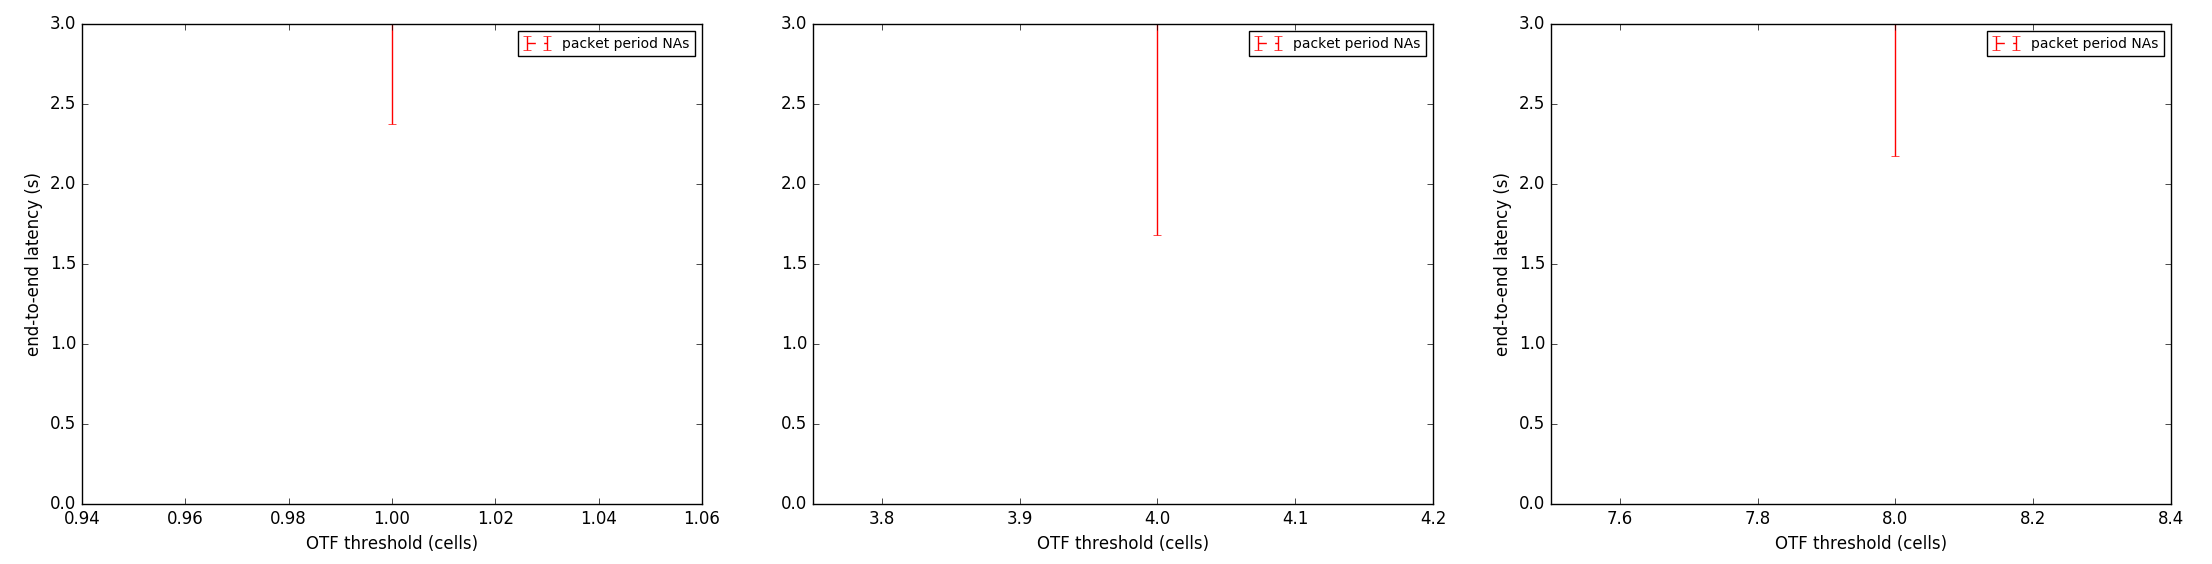
\includegraphics[width=1.0\textwidth]{lat_vs_threshold.png}
        \caption{Lat. vs umbral de 1, 4, y 8 respectivamente}
        \label{latvumbral1}
        \end{figure}


    En las figura \ref{latvumbral1} se muestra las diferencias entre el comportamiento de la latencia según el umbral que se contemple, el umbral que mejor desempeño entrega es con el umbral de cuatro.

\subsection{Latencia versus tiempo}

        \begin{figure}[h]
        \graphicspath{ {imagenes/agrupadas/} }
        \centering
        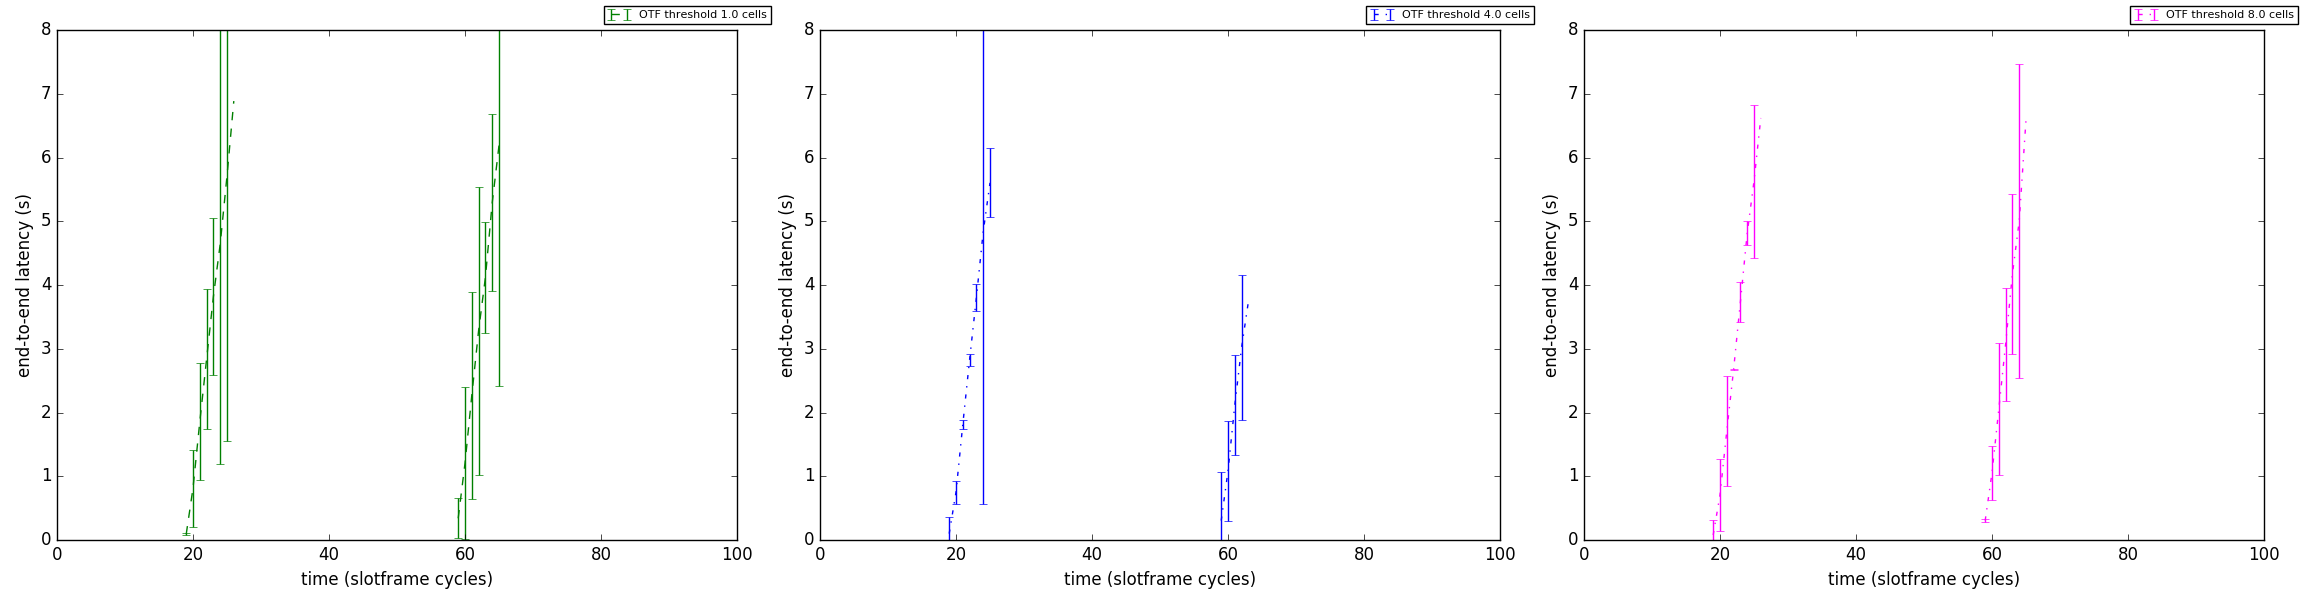
\includegraphics[width=1.0\textwidth]{latvtime.png}
        \caption{Lat. vs tiempo con umbral de 1, 4, y 8 respectivamente}
        \label{latvtime}
        \end{figure}

    Cuando se estudia el comportamiento de la latencia versus el tiempo, graficada en las imágenes agrupadas según umbral \ref{latvtime}. Es posible notar que a mayor umbral, menor propagación de latencia, esto hace sentido, ya que asignar y borrar celdas implican un consumo de tiempo el cual es el requisito de calcular celdas a operar. Es por esto, que la celda con umbral de uno propaga mayor latencia, ya que debe recalcular en mas ocasiones la cantidad de celdas a asignar.
    
    Las asignaciones de celdas versus unidad de tiempo, se pueden ver ampliadamente en las imágenes
    
\subsection{Actividad OTF de celdas versus tiempo}

        \begin{figure}[h]
        \graphicspath{ {imagenes/agrupadas/} }
        \centering
        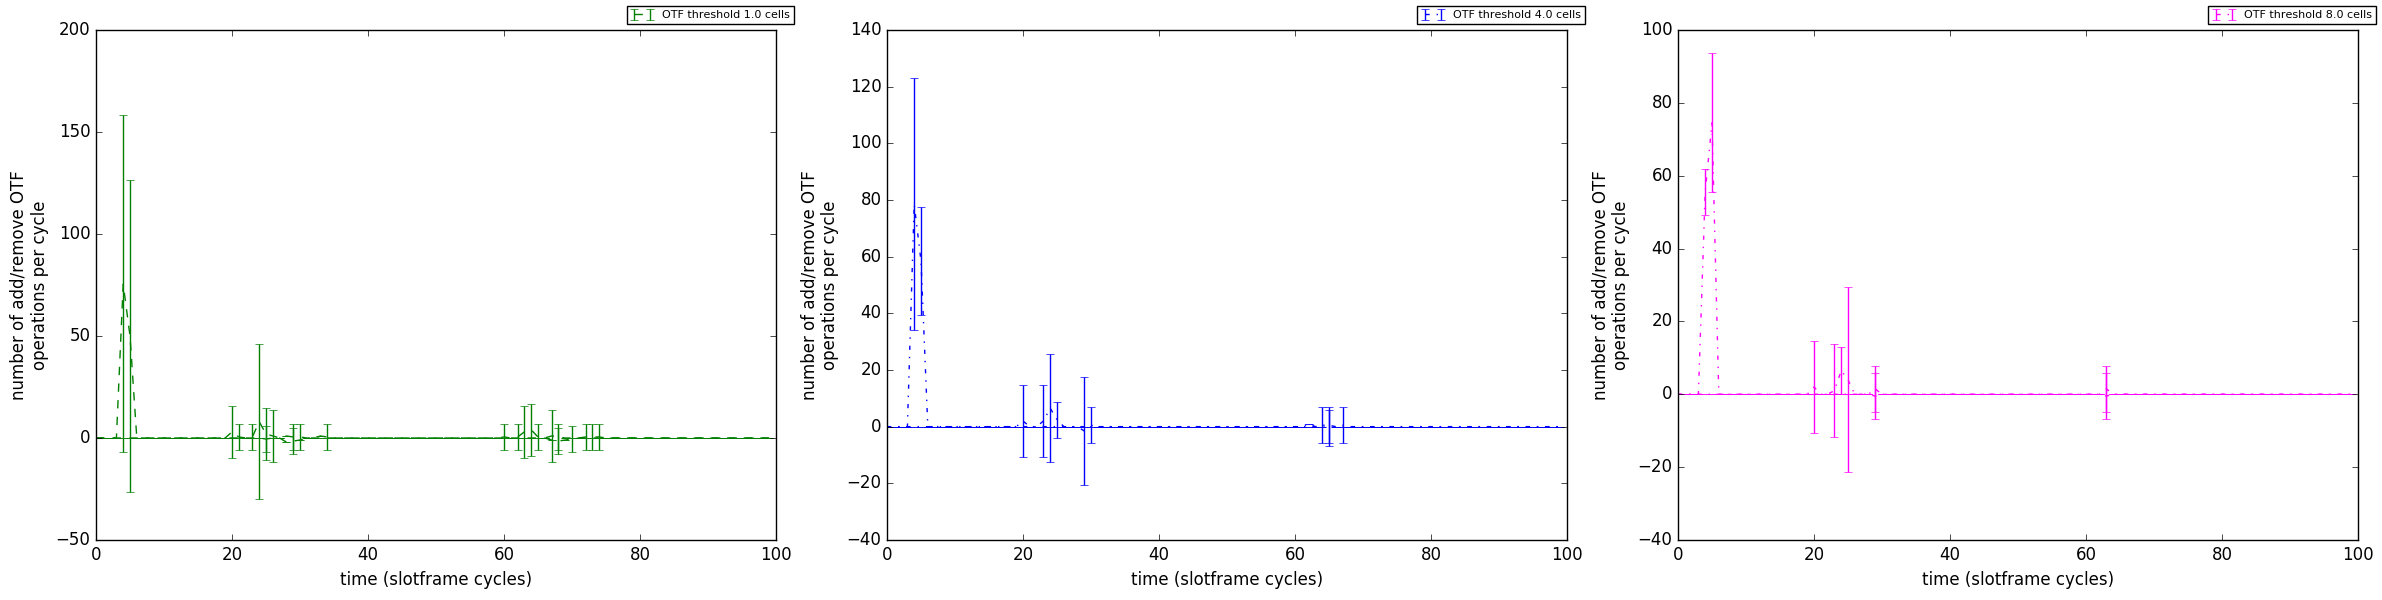
\includegraphics[width=1.0\textwidth]{otfactvstime.png}
        \caption{Activ. OTF con umbral de 1, 4, y 8 respectivamente}
        \label{actotfvtime}
        \end{figure}


    Analizando la actividad ``on the fly'' mostrada en las imágenes \ref{actotfvtime}, es evidente la diferencia del comportamiento según umbral, y que mientras mayor sea el umbral seleccionado, menor será la cantidad de movimientos de asignaciones de celdas de comunicación. Esto es una ventaja, ya que con esto se reduce el consumo energético implicado a las reasignaciones, pero por otro lado, un umbral demasiado grande implica un aumento de latencia, y un consumo excesivo de celdas.
    


\subsection{Número de celdas versus umbral}

        \begin{figure}[h]
        \graphicspath{ {imagenes/agrupadas/} }
        \centering
        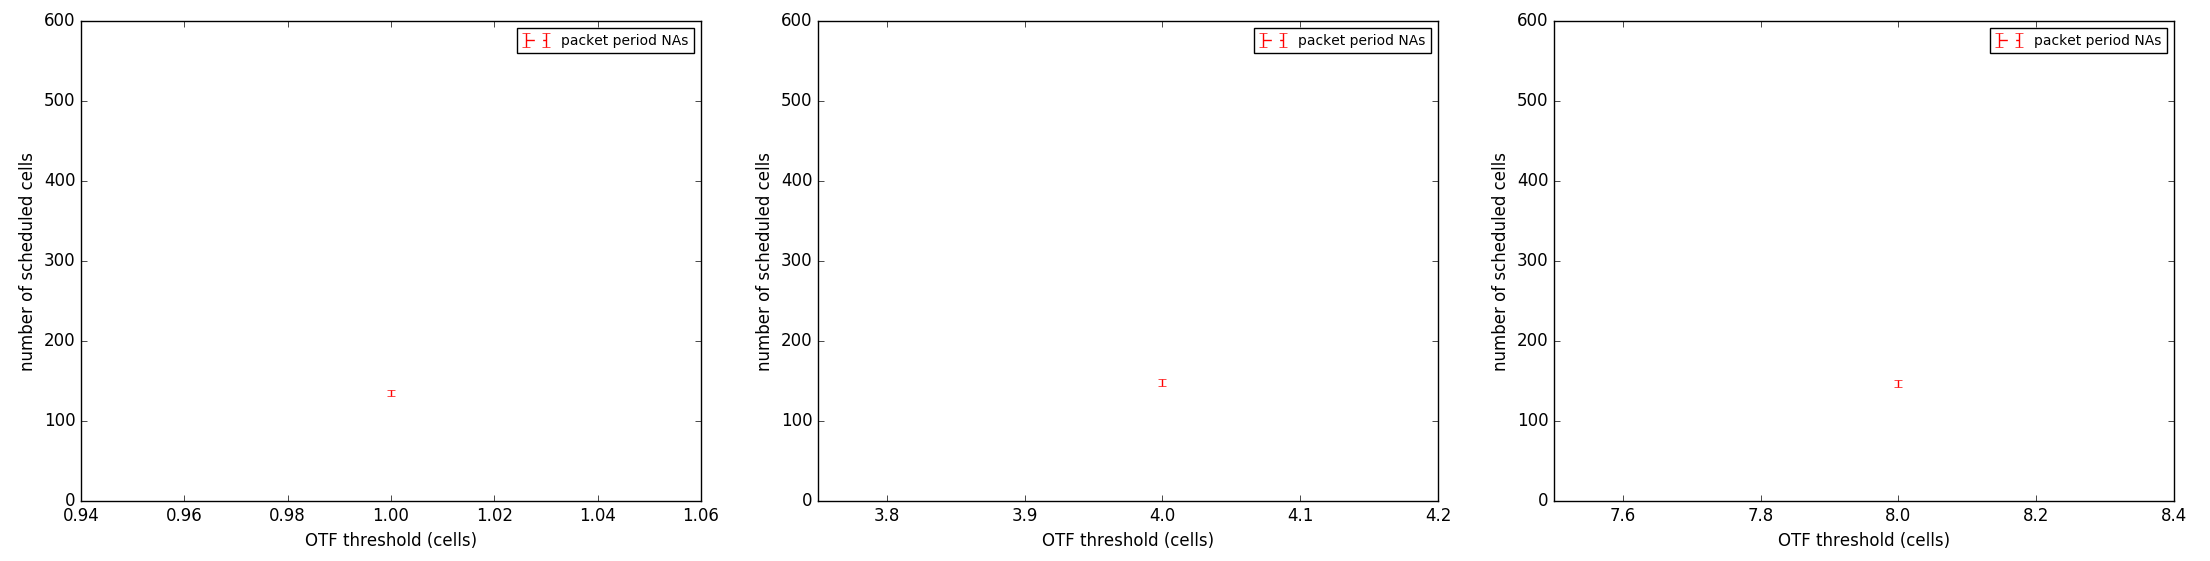
\includegraphics[width=1.0\textwidth]{numcelvsthre.png}
        \caption{Num. de celdas con umbral de 1, 4, y 8 respectivamente}
        \label{numcelvthr}
        \end{figure}

    La cantidad de celdas asignadas reactivamente según umbral tiende a llegar a un equilibrio, en las imágenes \ref{numcelvthr}se puede apreciar que: en la simulación con un umbral de una celda, se tiene una cifra aproximada de ciento veinticinco celdas asignadas, pero al analizar la cifra obtenida por las simulaciones con un umbral de cuatro y ocho, se obtuvo una cifra similar, de alrededor de ciento cincuenta celdas, por lo tanto se puede deducir que se encontró una cifra de equilibrio.


\subsection{Actividad OTF versus umbral}

        \begin{figure}[h]
        \graphicspath{ {imagenes/agrupadas/} }
        \centering
        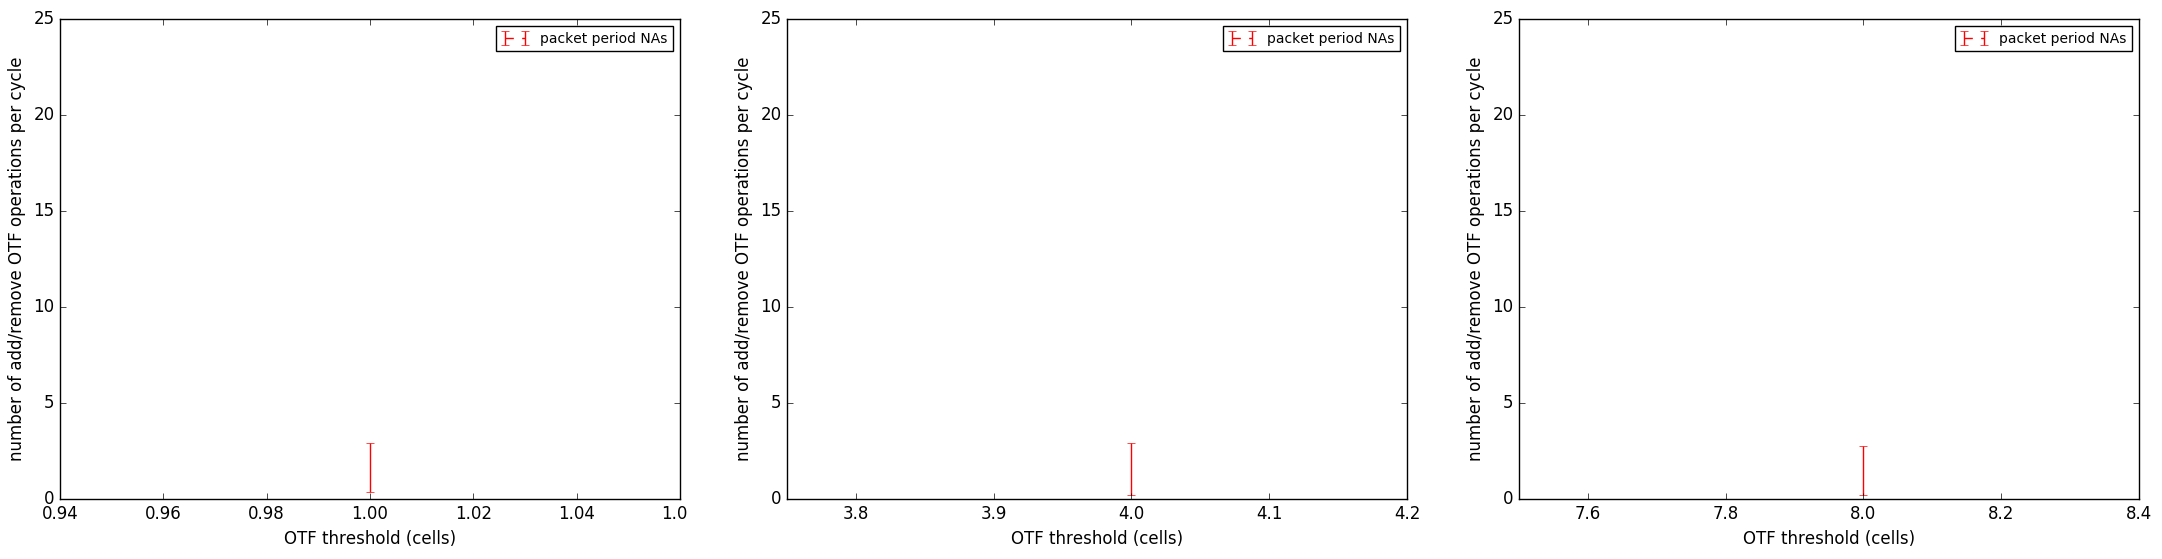
\includegraphics[width=1.0\textwidth]{otfactvthr.png}
        \caption{Act. OTF con umbral de 1, 4, y 8 respectivamente}
        \label{otfactvthr}
        \end{figure}

    La cantidad de operaciones de asignación y eliminado de celdas, tiene un comportamiento similar para cada umbral, las imágenes \ref{otfactvthr} dan cuenta de esto. Por lo tanto con esta información no es posible extraer ninguna conclusión, ya que no hay cambios significativos mas que muy leves diferencias, las cuales pueden ser adjudicadas a factores externos.

\subsection{Comparación de actividad OTF versus tiempo}

        \begin{figure}[h]
        \graphicspath{ {imagenes/agrupadas/} }
        \centering
        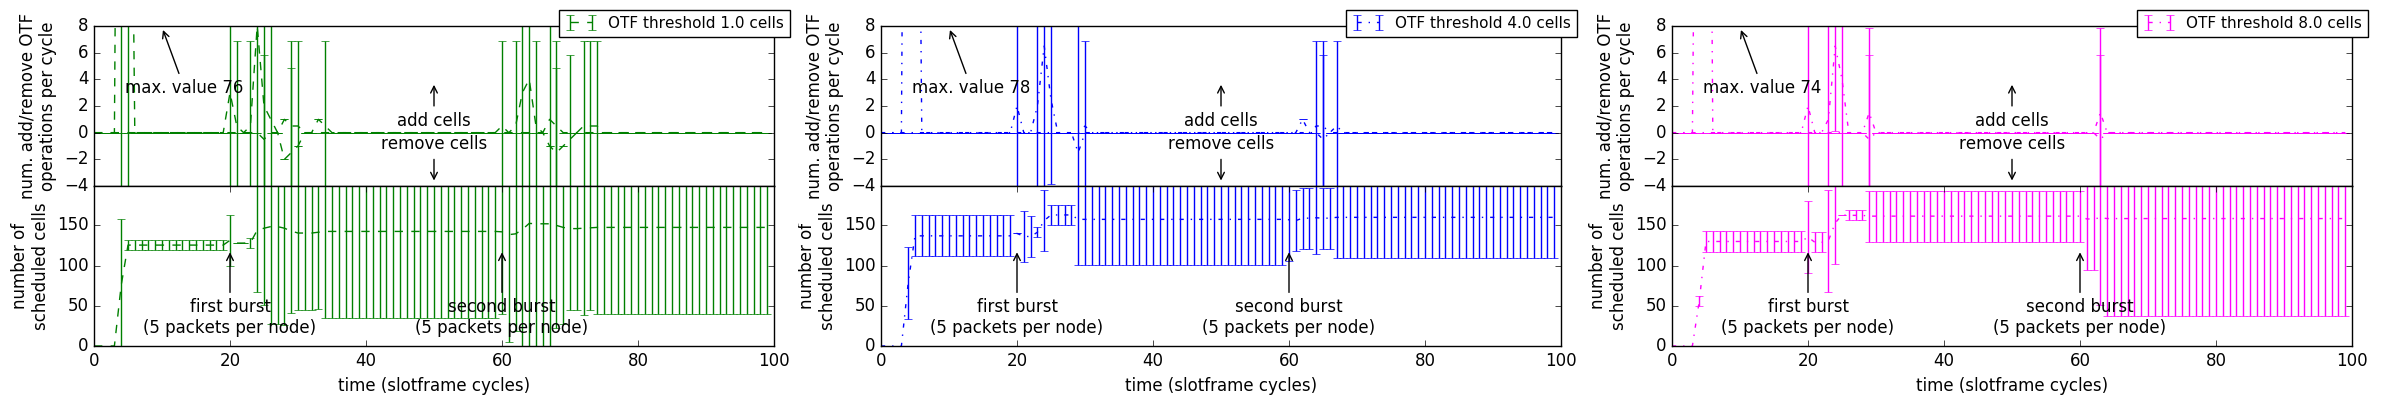
\includegraphics[width=1.0\textwidth]{numcellsotfactivtime.png}
        \caption{Act. OTF vs tiempo con umbral de 1, 4, y 8 respectivamente}
        \label{otfcomp}
        \end{figure}


    Esta sección es crítica, ya que en este momento se ve reflejado el efecto de las diferencias de umbral según sea el caso. Las imágenes \ref{otfcomp} muestra las diferencias en la cantidad de actividad de asignación-borrado de celdas según tamaño de umbral. Esto es coherente con el punto que trata la actividad OTF de celdas versus tiempo, y permite ver en detalle la cantidad de operaciones de asignación-eliminación.
    


\section{Resultados}
    
Tras analizar la información de los gráficos obtenidos utilizando el simulador, se puede observar que la variación del umbral en ciertos gráficos puede mostrar una mejora en el desempeño, pero que no se refleja en el proceso completo, por lo tanto analizar un solo gráfico no permite tener una información completa y representativa.
Es necesario trabajar con todas las variables según el escenario al que se esté enfrentando. Y recopilar información respecto al lugar hipotético donde se desee situar una malla de sensores, para que junto a un estudio del lugar, permita tomar la mejor decisión respecto a los parámetros con los que trabajarán los nodos.
% incluya otros archivos según su necesidad
% \input{archivo}
\chapter[]{}
\label{ch:conclu}

\section{Conclusión}

Hoy en día el protocolo IP se ha transformado en la columna vertebral de las redes mundiales, pero por sobre todo internet. Este protocolo, junto a una importante normalización realizada por la IETF es que los estándares como 6LoWPAN dan cabida a que los dispositivos inalámbricos de bajo consumo puedan conectarse a internet, como cualquier otra máquina y formar un entorno participativo, lo que simplificaría enormemente la integración de las distintas tecnologías inalámbricas de bajo consumo en un sistema más complejo.

Las tecnologías de bajo consumo TSCH han probado ser capaces de satisfacer los estrictos requisitos de las aplicaciones industriales, por lo tanto han logrado convertirse en parte fundamental de los estándares “WirelessHART”, “ISA100.11a”, y IEEE802.15.4e.

El objetivo de estas estandarizaciones es reducir el espacio entre las mas modernas redes TSCH y el estándar IETF, además de lograr que las redes inalámbricas sean capaces no solo de ser inalámbricas, sino también usar el protocolo IP versión 6, lo que abre una nueva forma de implementar redes TSCH. La implementación del protocolo IP versión 6 en una red TSCH da origen a las redes 6TiSCH. Con esto, las aplicaciones industriales se enfocarán en integrar la información extraída de distintos equipos, monitorear las tecnologías de operaciones, y permitir el uso de un modelo de capas común para permitir la comunicación ininterrumpida entre distintos equipos de distinta naturaleza, desde enormes equipos industriales, hasta pequeños nodos inalámbricos, todo esto dentro de una sola malla.

Para comenzar a trabajar con el protocolo 6TiSCH, se hizo necesario conocer sus capacidades, fortalezas y debilidades. Es por esto, que se trabajó con un simulador, que permitió estudiar el comportamiento del protocolo bajo un escenario. Se usaron distintas configuraciones para comparar las diferencias en el desempeño del simulador bajo un mismo escenario.

Luego de haber realizado la simulación utilizando 6TiSCH simulator, se obtuvo información importante respecto al funcionamiento y el desempeño del sistema de asignación de celdas en una malla de sensores. Esta información consistente en gráficas, se agrupó, y se comparó según las distintas configuraciones para un mismo evento.


Analizando la información obtenida, es posible comprender que tanto las topologías, cómo las configuraciones de los nodos influyen directamente en como la información es propagada hacia la fuente. Cuando nos enfocamos en el comportamiento de la latencia, es posible notar que aumenta directamente según la cantidad de nodos presentes en la malla. Por otro lado, cuando analizamos el tamaño de las colas de los sensores, se aprecia que una cola muy extensa aumenta la latencia final, además de requerir mas operaciones de eliminación. Por otro lado, una cola muy corta exige eliminar y reasignar continuamente celdas nuevas, lo que implica un alto consumo energético, reduciendo la vida de las baterías.

Es necesario ajustar los parámetros de los nodos a cada requerimiento, para conseguir el desempeño más cercano al óptimo. Esto se consigue estudiando el escenario que se utilizará, además de realizar mediciones de cobertura, interferencia, relación señal ruido.

Se espera que este trabajo investigación culmine con la obtención de un algoritmo de asignación de celdas con mejor desempeño respecto a los existentes hoy en día.


% Iniciamos el resto de secciones adicionales al contenido: referencias y apendices
\backmatter


% Bibliografía
% referencias.bib es el archivo con la base de datos bibliografica
% se recomienda utilizar un manejador de referencias: Jabref (jabref.sourceforge.net)
% El estilo por defecto es IEEE Transactions
\bibliographystyle{IEEEtran}
% Acá puede incluir uno más archivos de referencia
\bibliography{IEEEabrv,referencias}


% Simbología y glosario
% Utilice un paquete para generar símbolos y glosarios.
% Por ejemplo: nomencl (http://texdoc.net/pkg/nomencl)


% Anexos
\appendix

% Aca se incluyen los archivos con el texto de los anexos
% Por ejemplo, anexo.tex
\chapter{Primer anexo}
\label{ch:anexo-a}


% puede incluir más archivos de anexos
% \input{anexo-dos}

\end{document}
% that's all folks